\begin{pastexam}[label={px:ccu-113-swa-01}]{中正資工所甲組 113 學年度 第 1 題}
（單選）

The following is an AVL tree, which is implemented/represented as an array. Please answer the following questions from Q1 to Q3.

\begin{center}
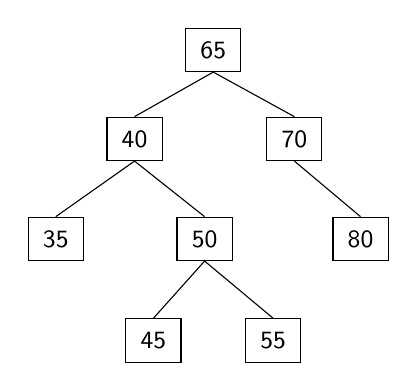
\begin{tikzpicture}[font=\sffamily\small]
\node[draw,rectangle,minimum width=7mm,minimum height=5.5mm,inner sep=1pt] (a) at (7.08,-5.92) {65};
\node[draw,rectangle,minimum width=7mm,minimum height=5.5mm,inner sep=1pt] (b) at (6.08,-7.05) {40};
\node[draw,rectangle,minimum width=7mm,minimum height=5.5mm,inner sep=1pt] (c) at (8.11,-7.05) {70};
\node[draw,rectangle,minimum width=7mm,minimum height=5.5mm,inner sep=1pt] (d) at (5.08,-8.32) {35};
\node[draw,rectangle,minimum width=7mm,minimum height=5.5mm,inner sep=1pt] (e) at (6.97,-8.32) {50};
\node[draw,rectangle,minimum width=7mm,minimum height=5.5mm,inner sep=1pt] (f) at (8.95,-8.32) {80};
\node[draw,rectangle,minimum width=7mm,minimum height=5.5mm,inner sep=1pt] (g) at (6.32,-9.61) {45};
\node[draw,rectangle,minimum width=7mm,minimum height=5.5mm,inner sep=1pt] (h) at (7.84,-9.61) {55};
\draw (a.south)--(b.north) (a.south)--(c.north) (b.south)--(d.north) (b.south)--(e.north) (c.south)--(f.north) (e.south)--(g.north) (e.south)--(h.north);
\end{tikzpicture}
\end{center}

(3\%) After inserting a new node with the key "43" into the AVL tree, what does the array representation of the AVL tree look like? Please note that a "$-$" represents a null value in the array.
\begin{enumerate}[label=\Alph*.]
\item (65, 40, 70, 35, 50, $-$, 80, $-$, $-$, 45, 55, $-$, 43)
\item (65, 40, 70, 35, 45, $-$, 80, $-$, $-$, 43, 50, $-$, $-$, 55)
\item (65, 45, 70, 40, 50, $-$, 80, 35, 43, $-$, 55)
\item (65, 45, 70, 35, 50, $-$, $-$, 80, 40, 43, $-$, 55)
\item None of the above
\end{enumerate}
\end{pastexam}

\begin{pastsoln}
答案是 C。

照資結書第~10.2.3~節：先照二元搜尋樹插入，再從新節點往根走，找第一個平衡因子變成 $\pm 2$ 的節點。
樹用「根(左子樹, 右子樹)」表示，$-$ 是空的子樹；平衡因子是左子樹高減右子樹高。

\textbf{插入。} $43 < 65$ 往左，$43 > 40$ 往右，$43 < 50$ 往左，$43 < 45$ 往左，接成 $45$ 的左子節點。

\textbf{往上檢查。} $45$ 的平衡因子 $+1$；$50$ 的左子樹（$45$、$43$）高 $2$、右子樹（$55$）高 $1$，是 $+1$；
$40$ 的左子樹（$35$）高 $1$、右子樹（以 $50$ 為根）高 $3$，是 $-2$，失衡，$A = 40$。

\textbf{旋轉。} 新節點在 $A$ 的右子節點 $50$ 的\textbf{左}子樹裡，是 RL：先對 $50$ 右旋、再對 $40$ 左旋，$45$
升到 $40$ 原來的位置。 $45$ 原來的左子樹（$43$）改掛到 $40$ 的右邊，右子樹（空）改掛到 $50$ 的左邊：
\[
40\bigl(35, 50(45(43, -), 55)\bigr) \ \Longrightarrow\ 45\bigl(40(35, 43), 50(-, 55)\bigr).
\]
這一段的高度回到插入前的 $3$，$65$ 的平衡因子也回到 $+1$，不必再轉。 整棵樹：
\begin{center}
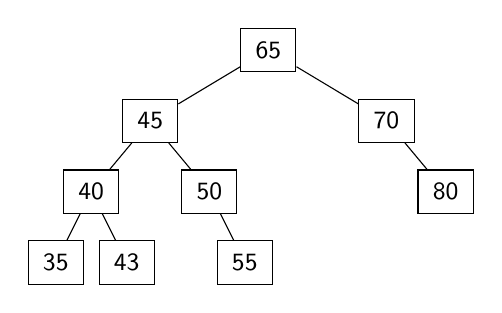
\begin{tikzpicture}[v/.style={draw,rectangle,minimum width=7mm,minimum height=5.5mm,inner sep=1pt,font=\sffamily\small},
  level distance=9mm, level 1/.style={sibling distance=30mm}, level 2/.style={sibling distance=15mm},
  level 3/.style={sibling distance=9mm}]
\node[v] {65}
  child {node[v] {45}
    child {node[v] {40} child {node[v] {35}} child {node[v] {43}}}
    child {node[v] {50} child[missing] child {node[v] {55}}}}
  child {node[v] {70} child[missing] child {node[v] {80}}};
\end{tikzpicture}
\end{center}
用陣列表示（資結書第~7.2.1~節）：第 $i$ 格的左右子節點在第 $2i$、$2i + 1$ 格。 第 $1$--$3$ 格 $65, 45, 70$；
第 $4$--$7$ 格是 $45$ 的子節點 $40, 50$ 和 $70$ 的子節點（空、$80$）；第 $8$--$11$ 格是 $40$ 的子節點
$35, 43$ 和 $50$ 的子節點（空、$55$）：
\[
(65, 45, 70, 40, 50, -, 80, 35, 43, -, 55),
\]
就是 C。

逐項檢查：
\begin{itemize}
\item A：沒有旋轉，$40$ 仍然失衡；而且 $43$ 放在第 $13$ 格，那是第 $6$ 格（空的）的右子節點。 只做二元
搜尋樹的插入時，$43$ 是 $45$ 的左子節點，應該在第 $20$ 格。 錯。
\item B：第 $14$ 格是第 $7$ 格（$80$）的左子節點，等於把 $55$ 放進 $65$ 的右子樹，但 $55 < 65$，連二元搜尋樹
都不是。 錯。
\item C：上面的結果。 對。
\item D：第 $4$ 格放 $35$、第 $8$ 格放 $80$，$80$ 變成 $35$ 的左子節點，連二元搜尋樹都不是。 錯。
\item E：C 是對的。 錯。
\end{itemize}
\end{pastsoln}
